\chapter{Evaluation}
\label{chp:Evaluation}

In this thesis a novel approach to the construction of uniform, consistent, and interoperable task-specific languages for model management has been proposed. This chapter provides an evaluation of the research hypothesis stated in Section \ref{sec:Analysis.Hypothesis}, the process that was followed to investigate it, and of the obtained research results, from several viewpoints. In Section \ref{sec:Evaluation.CaseStudy}, an extensive case study that requires use of a number of languages developed in this thesis is presented. The aim of the case study is to demonstrate the engineering qualities and practicality of the proposed solution. The description of the case study was set up by the organizers of the Model Driven Tools Implementers Forum (MDD-TIF) \cite{MDDTIF} in 2007, and besides the implementation using Epsilon, a number of additional implementations using state-of-the-art MDE tools and languages were presented during the workshop \cite{MDDTIF}.

In Section \ref{sec:Evaluation.Impact}, the impact of the work on the Model Driven Engineering community is assessed. Several factors are taken into consideration for this purpose; namely, the publications produced as a result of this work and their visibility, the acceptance and visibility of the proposed solution in the MDE community, and the exploitation of the research outcome in the context of the ModelWare and ModelPlex research projects.

Section \ref{sec:Evaluation.Reuse} demonstrates the benefits, in terms of reuse, delivered by the layered nature of the proposed architecture. Reuse is measured in terms of the size of the code required to implement the concrete syntax, execution engine and development tools of each language in the platform. Section \ref{sec:Evaluation.Limitations} discusses the limitations and shortcomings of this work; most notably the absence of mathematically expressed formal semantics. Section \ref{sec:Evaluation.ReferenceImplementation} evaluates the qualities of the reference implementation and provides directions for its evolution.

\section{Case Study}
\label{sec:Evaluation.CaseStudy}

This section presents a case study that uses combinations of languages of the Epsilon platform to implement a number of model management tasks. The scenario and requirements of the case study have been defined by the organizers of the Model Driven Development Tools Implementers Forum (MDD-TIF) \cite{MDDTIF} to enable a comparison of several different MDE tools using a common basis.

\subsection{Scenario}

The following case study description has been taken as-is from the MDD-TIF web-site \cite{MDDTIF}.

\subsubsection{Abstract}
Digital television allows interactive content to accompany standard broadcasts. The development of bespoke interactive content is expensive. You are to design a system that will allow the non-technical producers of television programmes to build interactive content from a set of high-level building blocks.
In effect, you will create a modelling language (metamodel, rules and symbols), a tool supporting it, and a generator.

\subsubsection{Background}
Digital television is becoming increasingly popular in the UK. In addition to providing higher quality video and increased channel capacity, it allows interactive content to accompany standard broadcasts. Interactive applications have been used to enhance traditional broadcasts in many ways:

\begin{itemize}
	\item Viewers can play along with quizzes (Figure \ref{fig:MDDTIFFigure1}).
	\item Viewers can choose different camera angles during sporting events
	\item Viewers can take part in discussions and comment on events though message boards.
	\item Viewers can remind themselves of the important developments in a drama's plot (Figure \ref{fig:MDDTIFFigure2}).
\end{itemize}

\begin{figure}
	\centering
		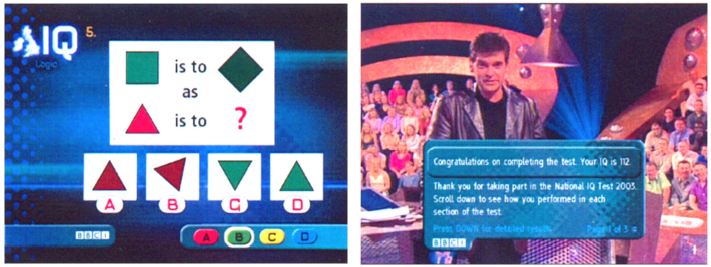
\includegraphics[width=1\textwidth]{images/MDDTIFFigure1.png}
	\caption{Playing along with Test the Nation}
	\label{fig:MDDTIFFigure1}
\end{figure}

\begin{figure}
	\centering
		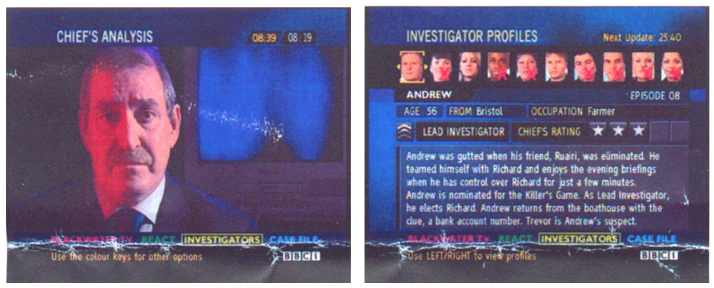
\includegraphics[width=1\textwidth]{images/MDDTIFFigure2.png}
	\caption{Viewing developments in The Murder Game}
	\label{fig:MDDTIFFigure2}
\end{figure}

\subsubsection{Problem}
Currently, each interactive application is bespoke. This greatly limits the number of programmes that can be accompanied by interactive content, as the applications are expensive to develop. The resulting UI is also different for different programmes, which is confusing to users. You are to design a system that will allow non-technical producers to build applications to accompany their programmes.

The application will sit on the right hand side of the screen (Figure \ref{fig:MDDTIFFigure3}), and display one of the following pieces of content:

\begin{itemize}
	\item A page of text, to be used for news stories, background information etc.
	\item A multiple choice vote, for example \emph{Man of the match} in a football match.
	\item A menu that allows the user to view items of content, including sub-menus.
\end{itemize}

The basic on-screen layout and navigational structure of the application has been defined by the user experience department, and producers are not able to change it.

\begin{figure}
	\centering
		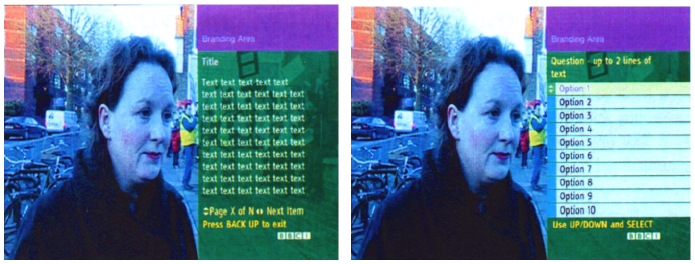
\includegraphics[width=1\textwidth]{images/MDDTIFFigure3.png}
	\caption{Different types of content}
	\label{fig:MDDTIFFigure3}
\end{figure}

\subsubsection{Use cases}
The following set of use cases emerged during discussions with the producers. They are ordered by their value to the producers, with the use case giving the most value first.

\paragraph{Case 1}
A producer would like to build an application for the soccer world cup finals, listing the teams and information about each, and allowing viewers to vote for the most likely winner.

\paragraph{Case 2}
As Case 1, but the teams should be listed by group (e.g. four teams in three groups). As the
teams are known before their division into groups by lots, it should be possible to define the
content for the teams first, and quickly add the structure of the groups, so that the application
can be running for users as soon as possible during the program that broadcasts the division
by lots.

\paragraph{Case 3}
A producer would like to use a page of text to provide analysis of the recent events in a rugby
match. A journalist with a laptop will need to change the text on the page throughout the
match. The user interface used by the journalist should not allow him to change the structure
of the whole application, only edit the text.

\paragraph{Case 4}
A producer has decided that the wording of a particular text page was better before the last
set of changes, and would like to revert it.

\subsubsection{Interactive application architecture}
Designing interactive applications requires relatively detailed knowledge of the standards for
each platform. For this reason, you should concentrate on the system used by producers to
define the application content, and its interfaces to black box components that build the
actual application. To define these interfaces, you will need some knowledge of the basic
architecture of interactive applications. The following crash-course should suffice.
Digital televisions contain a basic operating system, and a set of libraries providing functions
to display text and graphics, change the currently displayed video stream, etc. Applications
are designed and specified with a domain-specific modelling language (that you develop)
and delivered to digital televisions by inserting it as XML into the same broadcast stream that
contains the video and audio content. Once running, an application can be updated by
changing the XML in the broadcast stream. Applications can send reply messages to your
system, usually via a standard modem built into the television. Sending these reply messages
is very slow, and involves the viewer paying call charges. For these reasons, reply
messages can only be used for viewer initiated actions, such as responding to a vote.

\subsubsection{Code generation}
You should generate code like the following as plain text, rather than using any special
method for saving models as XML. This puts the various tools on an even footing, and
demonstrates the code generation facilities better for all kinds of code and other output files.
Handling white space and encodings is not vital, but the results should be machine and
human-readable.

\begin{lstlisting}[float=tbp, basicstyle=\ttfamily\footnotesize, flexiblecolumns=true, numbers=none, nolol=true, caption=Sample Generated XML, label=lst:MDDTIFXML, language=XML, tabsize=2]
<TVApp name=�World Cup 2010�>
	<Menu name=�World Cup�>
		<Vote name=�Who will win?�>
			<Choice name=�Estonia�/>
			<Choice name=�Lithuania�/>
		</Vote>
		<Text name=�World Cup trivia�>Trinidad &amp; 
			Tobago were the first ...</Text>
		<Menu name=�Teams�>
		�
		</Menu>
	</Menu>
</TVApp>
\end{lstlisting}


\subsection{Solution}

The case study presented above is within the scope of Epsilon as it involves a number of different model management tasks such as model validation, model-to-model transformation, model merging and model-to-text transformation. Moreover, to implement some cases (e.g. the code generation case), more than one individual model management tasks need to be combined. This section demonstrates an implementation of the functional requirements (cases) discussed above using Epsilon languages combined using the workflow mechanism presented in Chapter \ref{chp:Workflow}. The aim of this implementation is to cover as many cases as possible in an integrated manner with minimal duplication of code.

\subsubsection{Designing the TVApp DSL}

The first step of the solution is to design a Domain Specific Language (DSL) that enables users to design Interactive TV Applications. The TVApp DSL has been specified atop EMF by defining its abstract syntax in terms of ECore (using Emfatic \cite{Emfatic} as a convenience textual representation). A graphical overview of the DSL is presented in Figure \ref{fig:TVApps}.

\begin{figure}
	\centering
		%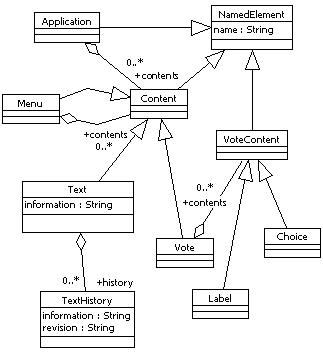
\includegraphics[width=0.45\textwidth]{images/TVApps}
		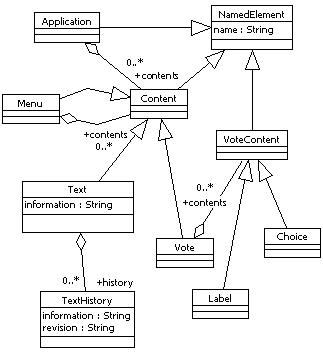
\includegraphics{images/TVApps}
	\caption{The TVApps Domain Specific Language}
	\label{fig:TVApps}
\end{figure}

\subsubsection{Generating a TVApp model for a Sports Competition}
\label{sec:Competition}

To address Case 1, a new Competition metamodel has been designed for capturing information about competitions, groups and participating teams. A graphical overview of the metamodel is displayed in Figure \ref{fig:Competition}. The design of the metamodel also satisfies the requirement of Case 2 for defining the team-related information first and then adding the teams into groups by modifying the \texttt{competitors} list of each group.

\begin{figure}
	\centering
		%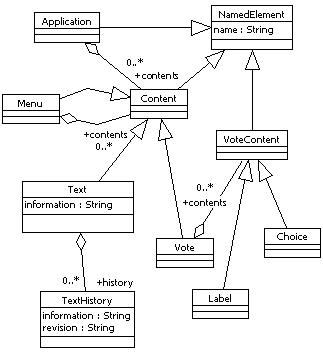
\includegraphics[width=0.45\textwidth]{images/TVApps}
		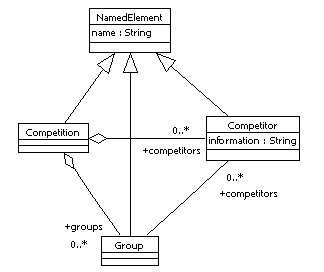
\includegraphics{images/Competition}
	\caption{The Competition Domain Specific Language}
	\label{fig:Competition}
\end{figure}

Before the Competition model can be transformed into a TVApp model, it should be validated against a number of constraints so that potential errors are detected at this level and not propagated to the TVApp model. In Listing \ref{lst:ValidateCompetition} an Epsilon Validation Language module is used for this purpose. The \emph{NameSpecified} constraint in line \ref{line:NameSpecified} specifies that all named elements (that is \emph{Groups} and \emph{Competitors}) must specify a non-empty name. Moreover, in line \ref{line:NotEmpty}, the \emph{NotEmpty} constraint applies to Groups and specifies that each group must have at least one competitor. Here it is worth noticing that in its guard, the \emph{NotEmpty} constraint requires that to apply to particular Group, the Group must first satisfy the \emph{NameSpecified} constraint presented above. Finally, in line \ref{line:InUniqueGroup}, the \emph{InUniqueGroup} constraint checks that each competitor only participates in one Group.

\begin{lstlisting}[float=tbp, basicstyle=\ttfamily\footnotesize, flexiblecolumns=true, numbers=left, nolol=true, caption=EVL module that validates a Competition model, label=lst:ValidateCompetition, language=EVL, tabsize=2]
context Competition!NamedElement {
	
	constraint NameSpecified { /*@\label{line:NameSpecified}@*/
		
		check : self.name.isDefined() and self.name.trim().length > 0
		
		message : self.eClass().name + " must provide a name"
		
	}
	
}

context Competition!Group {
	
	constraint NotEmpty { /*@\label{line:NotEmpty}@*/
		
		guard : self.satisfies("NameSpecified")
		
		check : self.competitors.size() > 0
		
		message : "Group " + self.name + " contains no competitors"
		
	}
	
}

context Competition!Competitor {
	
	constraint InUniqueGroup { /*@\label{line:InUniqueGroup}@*/
		
		guard : self.satisfies("NameSpecified")
		
		check : Competition!Group.allInstances.
			select(g|g.teams.includes(self)).size() <= 1
		
		message : "Competitor " + self.name + 
			" exists in more than one group."
	}
	
}
\end{lstlisting}

Having validated the input Competition mode, the Epsilon Transformation Language discussed in Section \ref{sec:ETL} is used to transform it into a TVApp model. The transformation displayed in Listing \ref{lst:TransformCompetition} defines that an \texttt{Application} and a \texttt{Vote} will be generated from each \texttt{Competition}, and that the \texttt{Vote} will contain a flattened sequence of \texttt{Label}s (one for each \texttt{Group}) and \texttt{Choice}s (one for each \texttt{Competitor} in the group).

\begin{lstlisting}[float=tbp, basicstyle=\ttfamily\footnotesize, nolol=true, flexiblecolumns=true, numbers=left, caption=ETL transformation that transforms a Competition model into a TVApp model, tabsize=2, label=lst:TransformCompetition, language=ETL]
rule Competition2Application
	transform c : Competition!Competition
	to a : TVApp!Application, v : TVApp!Vote {

	a.name = c.name + " Application";
	v.name = "Who will win the " + c.name + "?";	
	a.contents.add(v);
	
	for (g in c.groups) {
		v.contents.add(g.equivalent());
		for (memb in g.members) {
			v.contents.add(memb.equivalent());
		}
	}
}

rule Competitor2Choice
	transform co : Competition!Competitor
	to ch : TVApp!Choice {

	ch.name = co.name;
}

rule Group2Label
	transform g : Competition!Group
	to l : TVApp!Label {
	
	l.name = "Group " + g.name;
}
\end{lstlisting}

The two steps are combined into a composite task that validates and - if all constraints are satisfied - then transforms the Competition model using the workflow presented in Listing \ref{lst:TransformCompetitionWorkflow}. In lines \ref{line:LoadCompetitionTask} and \ref{line:LoadTVAppTask}, the involved models are loaded using the \emph{epsilon.loadModel} task. In line \ref{line:ValidateCompetitionTask} the Competition model is validated using the EVL module presented in Listing \ref{lst:ValidateCompetition}, and if all constraints are satisfied, in line \ref{line:TransformCompetitionTask}, it is transformed into a TVApp model using the ETL module presented in Listing \ref{lst:TransformCompetition}

\begin{lstlisting}[float=tbp, basicstyle=\ttfamily\footnotesize, flexiblecolumns=true, numbers=left, nolol=true, caption=Workflow that integrates the validation and transformation steps, label=lst:TransformCompetitionWorkflow, language=XML, tabsize=2]
<?xml version="1.0"?>
<project default="main">
	
	<epsilon.loadModel name="Competition" type="EMF"> /*@\label{line:LoadCompetitionTask}@*/
		<parameter name="modelFile" file="models/WorldCup.model"/>
		<parameter name="metamodelUri" value="CompetitionDsl"/>
		<parameter name="isMetamodelFileBased" value="false"/>
		<parameter name="readOnLoad" value="true"/>
	</epsilon.loadModel>
	
	<epsilon.loadModel name="TVApp" type="EMF"> /*@\label{line:LoadTVAppTask}@*/
		<parameter name="modelFile" file="models/TVApp3.model"/>
		<parameter name="metamodelUri" value="TVAppDsl"/>
		<parameter name="isMetamodelFileBased" value="false"/>
		<parameter name="readOnLoad" value="false"/>
	</epsilon.loadModel>

	<target name="main">

		<epsilon.evl src="ValidateCompetition.evl"> /*@\label{line:ValidateCompetitionTask}@*/
			<model ref="Competition"/>
		</epsilon.evl>		
		
		<epsilon.etl src="Competition2TVApp.etl"> /*@\label{line:TransformCompetitionTask}@*/
			<model ref="TVApp"/>
			<model ref="Competition"/>
		</epsilon.etl>
		
	</target>
	
</project>
\end{lstlisting}

\subsubsection{Integrating Live Reports}
\label{sec:LiveReports}

Case 3 requires that an external user must be able to update a particular text but not the structure of the application. To achieve this, the Report DSL presented in Figure \ref{fig:Report} has been designed. The rationale is that particular users can be only granted the permission to compose Report models which will then be used to automatically update the original application model via merging. To satisfy the requirement set in Case 4, when merging the original TVApp with a Report, the original information contained in the \texttt{Text}s which the Report updates is not lost but instead is stored in the form of a new \texttt{TextHistory} model element. The merge has been specified using the ECL and EML languages modules displayed in Listings \ref{lst:CaseStudyEML} and \ref{lst:CaseStudyECL} respectively. An alternative to designing the one-metaclass Report DSL would be to add the Report class to the existing TVApp DSL. However, it was deemed more appropriate with regard to modularity and separation of concerns to establish a new (albeit minimal) DSL instead.

\begin{figure}
	\centering
		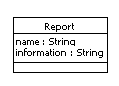
\includegraphics{images/Report}
	\caption{The Report Domain Specific Language}
	\label{fig:Report}
\end{figure}

As discussed in Section \ref{sec:EML}, EML operates in two steps. In the first step, correspondences are established between elements that need to be merged (using ECL or otherwise) and in the sequel corresponding elements are merged (using merge-rules) and non-matched elements are transformed into the target model (using transform-rules reused from ETL). In Listing \ref{lst:CaseStudyECL}, matching \texttt{Report}s from the Report model with \texttt{Text}s from an OldTVApp model is achieved through the \texttt{MatchReportWithText} ECL match-rule in line \ref{line:MatchReportWithText} that compares the names of the compared elements.

Then, in Listing \ref{lst:CaseStudyEML}, matching \texttt{Report}s and \texttt{Text}s are merged using the \texttt{MergeReportWithText} merge-rule in line \ref{line:MergeReportWithText} which specifies that the \texttt{Text} should be updated and that the old version of the text should be stored in the form of a new \texttt{TextHistory} model element with a proper information and revision number. The rest of the elements of the original TVApp model are copied to the target model using the transformation rules provided by the CopyTVApp module, displayed in Listing \ref{lst:CaseStudyCopyETL}, which is imported by the EML module using the \emph{import} statement in line \ref{line:ImportETL}.

\begin{lstlisting}[float=tbp, basicstyle=\ttfamily\footnotesize, flexiblecolumns=true, numbers=left, nolol=true, caption=ECL module that compares a TVApp with a Report model, label=lst:CaseStudyECL, language=ECL, tabsize=2]
rule MatchReportWithText /*@\label{line:MatchReportWithText}@*/
	match t : OldTVApp!Text
	with r : Report!Report {
	
	compare : r.name = t.name	
}
\end{lstlisting}

\begin{lstlisting}[float=tbp, basicstyle=\ttfamily\footnotesize, nolol=true, flexiblecolumns=true, caption=EML module that merges a TVApp with a Report model, tabsize=2, label=lst:CaseStudyEML, language=EML]
import "CopyTVApp.etl"; /*@\label{line:ImportETL}@*/

rule MergeReportWithText /*@\label{line:MergeReportWithText}@*/
	merge ot : OldTVApp!Text
	with r : Report!Report 
	into nt : NewTVApp!Text {
	
	nt.name = ot.name;
	nt.information = ot.information;
	nt.history ::= ot.history;
	
	var h : new NewTVApp!TextHistory;
	h.information = ot.information;
	h.revision = ot.history.collect(h|h.revision).max(0) + 1;
	nt.history.add(h);
	nt.information = r.information;
}
\end{lstlisting}

\begin{lstlisting}[float=tbp, basicstyle=\ttfamily\footnotesize, flexiblecolumns=true, numbers=left, nolol=true, caption=ETL transformation that copies a TVApp module, label=lst:CaseStudyCopyETL, language=ETL, tabsize=2]
rule CopyApplication
	transform s : OldTVApp!Application
	to t : Target!Application {
	
	t.name = s.name;
	t.contents ::= s.contents;
}
rule CopyText
	transform s : OldTVApp!Text
	to t : Target!Text {

	t.name = s.name;
	t.information = s.information;
	t.history ::= s.history;
}
rule CopyTextHistory
	transform s : OldTVApp!TextHistory
	to t : Target!TextHistory {

	t.revision = s.revision;
	t.information = s.information;
}
rule CopyVote
	transform s : OldTVApp!Vote
	to t : Target!Vote {

	t.name = s.name;
	t.contents ::= s.contents;
}
rule CopyChoice
	transform s : OldTVApp!Choice
	to t : Target!Choice {

	t.name = s.name;
}
rule CopyLabel
	transform s : OldTVApp!Label
	to t : Target!Label {

	t.name = s.name;
}
rule CopyMenu
	transform s : OldTVApp!Menu
	to t : Target!Menu {
	
	t.name = s.name;
	t.contents ::= s.contents;
}
\end{lstlisting}

In case a report in the Report model does not match a text in the TVApp model, the report is (correctly) not added into the target TVApp model. To inform the user about such cases, the EVL module of Listing \ref{lst:ValidateReport} is injected between the comparison and merging steps. The \emph{RefersToValidText} constraint specified in line \ref{line:RefersToValidText} examines the match-trace (\emph{trace}) established by the comparison step and requires that each report must match with a Text from the TVApp model.

\begin{lstlisting}[float=tbp, basicstyle=\ttfamily\footnotesize, flexiblecolumns=true, numbers=left, nolol=true, caption=EVL module that validates a Report model against a TVApp model, label=lst:ValidateReport, language=EVL, tabsize=2]
context Report!Report {
	
	constraint RefersToValidText { /*@\label{line:RefersToValidText}@*/
		
		check : trace.matches.exists(m|m.matching and m.right = self)
		
		message : "Report " + self.name + " refers to an undefined text"	
	}
}
\end{lstlisting}

The ECL, EVL and EML modules presented above are integrated using the workflow of Listing \ref{lst:CaseStudyMergingWorkflow}. In lines \ref{line:LoadReportTask}, \ref{line:LoadOldTVAppTask} and \ref{line:LoadNewTVAppTask} the involved models are loaded. In line 
\ref{line:MatchReportWithTVAppTask} the \emph{Report} model is compared with the \emph{OldTVApp} model using the ECL module of Listing \ref{lst:CaseStudyECL}

\begin{lstlisting}[float=tbp, basicstyle=\ttfamily\footnotesize, flexiblecolumns=true, numbers=left, nolol=true, caption=Workflow integrating the comparison\, validation and merging steps, label=lst:CaseStudyMergingWorkflow, language=XML, tabsize=2]
<?xml version="1.0"?>
<project default="main">
	
	<epsilon.loadModel name="Report" type="EMF"> /*@\label{line:LoadReportTask}@*/
		<parameter name="modelFile" file="models/Report.model"/>
		<parameter name="metamodelUri" value="ReportDsl"/>
		<parameter name="isMetamodelFileBased" value="false"/>
		<parameter name="readOnLoad" value="true"/>
	</epsilon.loadModel>
	
	<epsilon.loadModel name="OldTVApp" type="EMF"> /*@\label{line:LoadOldTVAppTask}@*/
		<parameter name="aliases" value="Source"/>
		<parameter name="modelFile" file="models/TVApp1.model"/>
		<parameter name="metamodelUri" value="TVAppDsl"/>
		<parameter name="isMetamodelFileBased" value="false"/>
		<parameter name="readOnLoad" value="true"/>
	</epsilon.loadModel>	
	
	<epsilon.loadModel name="NewTVApp" type="EMF"> /*@\label{line:LoadNewTVAppTask}@*/
		<parameter name="aliases" value="Target"/>
		<parameter name="modelFile" file="models/TVApp2.model"/>
		<parameter name="metamodelUri" value="TVAppDsl"/>
		<parameter name="isMetamodelFileBased" value="false"/>
		<parameter name="readOnLoad" value="false"/>
	</epsilon.loadModel>

	<target name="main">
		
		<epsilon.ecl src="MatchReportWithTVApp.ecl" 
			exportmatchtrace="trace"> /*@\label{line:MatchReportWithTVAppTask}@*/
			<model ref="OldTVApp"/>
			<model ref="Report"/>
		</epsilon.ecl>
		
		<epsilon.evl src="ValidateReport.evl"> /*@\label{line:ValidateReportTask}@*/
			<model ref="OldTVApp"/>
			<model ref="Report"/>
			<uses ref="trace"/>
		</epsilon.evl>
		
		<epsilon.eml src="MergeReportWithTVApp.eml" 
			usematchtrace="trace"> /*@\label{line:MergeReportWithTVAppTask}@*/
			<model ref="OldTVApp"/>
			<model ref="Report"/>
			<model ref="NewTVApp"/>
		</epsilon.eml>
		
		<epsilon.storeModel model="NewTVApp"/>
		
	</target>
	
</project>
\end{lstlisting}

\subsubsection{Generating XML from a TVApp model}
\label{sec:GeneratingXML}

To generate an XML document from a TVApp model, as required by the case study description, the intermediate XML metamodel displayed in Figure \ref{fig:XML} is used. Thus, the TVApp model is transformed into an XML model (Listing \ref{lst:TVApp2XML}) using the Epsilon Transformation Language, and then the textual representation of the XML model (Listing \ref{lst:EGL}) is generated using the Epsilon Generation Language. This approach promotes modularity and reuse by targeting XML-specific issues such as escaping and indentation in a separate transformation which can be reused as-is in other DSL to XML scenarios, and also complies with the requirement not to use a special (hard-coded) method for transforming XML models to text.

\clearpage

\begin{figure}
	\centering
		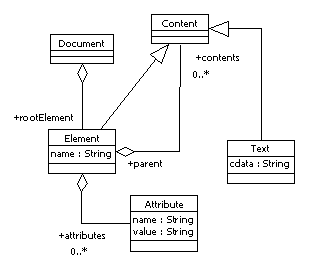
\includegraphics{images/XML}
	\caption{The XML Domain Specific Language}
	\label{fig:XML}
\end{figure}

\begin{lstlisting}[float=tbp, basicstyle=\ttfamily\footnotesize, nolol=true, flexiblecolumns=true, caption=ETL transformation that transforms TVApp models to XML models, tabsize=2, label=lst:TVApp2XML, language=ETL]
pre {
	var doc : new Xml!Document;
	doc.rootElement = TVApp!Application.
		allInstances.first().equivalent();
}

@abstract
rule NamedElement2Element
	transform ne : TVApp!NamedElement
	to n : Xml!Element {
	
	n.addAttribute("name", ne.name);
}

rule Application2Element
	transform a : TVApp!Application
	to n : Xml!Element extends NamedElement2Element{
	
	n.name = "Application";
	n.contents = a.contents.equivalent();
}

rule Vote2Element
	transform v : TVApp!Vote
	to n : Xml!Element extends NamedElement2Element {
	
	n.name = "Vote";	
	n.contents = v.contents.equivalent();
}

rule Choice2Element
	transform c : TVApp!Choice
	to n : Xml!Element extends NamedElement2Element {
	
	n.name = "Choice";	
}

rule Label2Element
	transform c : TVApp!Label
	to n : Xml!Element extends NamedElement2Element {
	
	n.name = "Label";
}

rule Text2Element
	transform t : TVApp!Text
	to e : Xml!Element extends NamedElement2Element {
	
	e.name = "Text";
	var text : new Xml!Text;
	text.cdata = t.information;
	e.contents.add(text);
}

rule Menu2Element
	transform m : TVApp!Menu
	to e : Xml!Element extends NamedElement2Element {
	
	e.name = "Menu";
	e.contents = m.contents.equivalent();
}

operation Xml!Element addAttribute
	(name : String, value : String) {
	var attr : new Xml!Attribute;
	attr.name = name;
	attr.value = value;
	self.attributes.add(attr);
}
\end{lstlisting}

The ETL transformation of Listing \ref{lst:TVApp2XML}, demonstrates two important characteristics of ETL: rule inheritance and state-changing operations. By inheriting from the abstract rule \textit{NamedElement2Element}, the rest of the rules are maintained simple and without duplication. Moreover, defining the \textit{addAttribute()} state-changing operation simplifies the \textit{NamedElement2Element} rule. 

\begin{lstlisting}[float=tbp, basicstyle=\ttfamily\footnotesize, nolol=true, flexiblecolumns=true, caption=EGL template that generates XML text from XML models, tabsize=2, label=lst:EGL, language=EOL]
<?xml version="1.0"?>
[%=Document.allInstances().first().rootElement.toString(0)%]

[%
operation Element toString(indent : Integer) : String {
	var str : String;
	str = indent.getIndent() + "<" + self.name.normalize();
	for (a in self.attributes) {
		str = str + " " + a.name.normalize() + 
			"='" + a.value.normalize() + "'";
		if (hasMore){
			str = str + " ";
		}
	}
	str = str + ">\r\n";
	for (c in self.contents) {
		str = str + c.toString(indent + 1);
	}
	str = str + indent.getIndent() + "</" + 
		self.name.normalize() + ">\r\n";
	return str;
}

operation Text toString(indent : Integer) : String {
	return (indent + 1).getIndent() + 
		self.cdata.normalize() + "\r\n";
}

operation Integer getIndent() : String {
	var indent : String;
	for (i in Sequence{1 .. self}){
		indent = indent + "  ";
	}
	return indent;
}

operation String normalize() {
	var normalized : String = self;
	if (not normalized.isDefined()) { 
		normalized = "";
	}
	else {
		normalized = normalized.replace("&", "&amp;");
		normalized = normalized.replace("<", "&lt;");
		normalized = normalized.replace(">", "&gt;");
		// etc
	}
	return normalized;
}
%]
\end{lstlisting}

Generating XML text from an XML model in Listing \ref{lst:EGL} involves much dynamic and little static text. Therefore, the vast majority of the serialization process is performed via string concatenation. By contrast, the header (processing instruction and comment) is only static text that is emitted as-is from the template.

\subsubsection{Integrating the Model-to-Model and the Model-to-Text steps}

To integrate the two steps presented above into a coherent process that transforms a TVApp model directly to textual XML, the Epsilon Workflow is used. Thus, in Listing \ref{lst:CaseStudyCodeGenWorkflow}, two tasks for loading the involved models (epsilon.loadModel), one that invokes the ETL transformation (epsilon.etl) and one that invokes the EGL model-to-text transformation on the intermediate XML model (epsilon.egl) are used.

\begin{lstlisting}[float=tbp, basicstyle=\ttfamily\footnotesize, nolol=true, numbers=left, flexiblecolumns=true, caption=The workflow that integrates the ETL and EGL tasks, tabsize=2, label=lst:CaseStudyCodeGenWorkflow, language=XML]
<?xml version="1.0"?>
<project default="main">
	
	<epsilon.loadModel name="TVApp" type="EMF">
		<parameter name="modelFile" file="models/ChampionsLeague.model"/>
		<parameter name="metamodelUri" value="TVAppDsl"/>
		<parameter name="isMetamodelFileBased" value="false"/>
		<parameter name="readOnLoad" value="true"/>
	</epsilon.loadModel>
	
	<epsilon.loadModel name="Xml" type="EMF">
		<parameter name="modelFile" file="models/TVAppXml.model"/>
		<parameter name="metamodelUri" value="Xml"/>
		<parameter name="isMetamodelFileBased" value="false"/> 
		<parameter name="readOnLoad" value="false"/>
	</epsilon.loadModel>

	<target name="main">

		<epsilon.etl src="TVApp2Xml.etl">
			<model ref="TVApp"/>
			<model ref="Xml"/>
		</epsilon.etl>
		
		<epsilon.egl src="Xml2Text.egl" target="output/TVApp.xml">
			<model ref="Xml"/>
		</epsilon.egl>
	</target>
</project>
\end{lstlisting}

\subsubsection{Generating a Mock-up of the TV Application}
\label{sec:Mockup}

A feature that is not required explicitly by the case study description, but which was regarded as particularly useful is to be able to \textit{preview} a TVApp model using a mock-up that closely resembles the appearance of the final deployed application. Therefore, EGL has been used to compose a model-to-text transformation that generates a set of linked HTML screens that emulate the look-and-feel and functionality of the deployed application. Listing \ref{lst:Mockup} presents the main template of the EGL solution that iterates the model and invokes the respective sub-templates (Text.egl, Menu.egl, Vote.egl) to generate the mockup HTML screens.

\begin{lstlisting}[float=tbp, basicstyle=\ttfamily\footnotesize, nolol=true, flexiblecolumns=true, caption=EGL template that generates mockup HTML screens for a TVApp model, tabsize=2, label=lst:Mockup, language=EOL]
[%
	import "include\\Common.eol";

	TemplateFactory.setTemplateRoot("workspace\\MDD-TIF");
	TemplateFactory.setOutputRoot("workspace\\MDD-TIF\\html");
	
	var header : Template = 
		TemplateFactory.load("include\\Header.egl");
	var text : Template = 
		TemplateFactory.load("include\\Text.egl");	
	var menu : Template = 
		TemplateFactory.load("include\\Menu.egl");
	var vote : Template = 
		TemplateFactory.load("include\\Vote.egl");
	var footer : Template = 
		TemplateFactory.load("include\\Footer.egl");
	
	var contents : String = "default";
	
	if (Application.isType(content) or Menu.isType(content)) {
		menu.populate("menu", content);
		contents = menu.process();
		
		// Recursively generate the pages 
		// for the contents of this
		// application / menu
		for (child in content.contents) {
			var page : Template = TemplateFactory.load("Page.egl");
		
			page.populate("content", child);
			
			page.generate(child.filename());
		}

	} else {
		if (Text.isType(content)) {
			text.populate("text", content);
			contents = text.process();

		} else {
			if (Vote.isType(content)) {
				vote.populate("vote", content);
				contents = vote.process();
			}
		}
	}
	
%]
[%=header.process()%]
[%=contents%]
[%=footer.process()%]
\end{lstlisting}

%\subsection{Other Submitted Solutions}

%Is this worth writing?

\subsection{Summary}

The case study presented in this section involves four different model management tasks, three of which comprise of more than one step, for each of which a different model management language is more appropriate. Table \ref{tab:CaseStudyMatrix} provides an overview of the tasks and the languages involved in providing a solution for each one.

\begin{table}
	\centering
		\begin{tabular}{|l|l|l|}\hline
			\textbf{Task} & \textbf{Languages used} \\\hline
			Transform a Competition into a TVApp model & EVL, ETL \\\hline
			Provide Support for Live Reports & ECL, EVL, EML \\\hline
			Generate XML from a TVApp model & ETL, EOL \\\hline
			Generate Mock-up screens from a TVApp model & EGL \\\hline
		\end{tabular}
	\caption{Matrix of Tasks and applied Languages}
	\label{tab:CaseStudyMatrix}
\end{table}

The solution has demonstrated that the layered architecture proposed in this work enables users to decompose complex tasks into steps that are easily manageable with one of the task-specific languages provided and then exploit the inherent interoperability of the individual languages to compose the steps into coherent composite tasks using the proposed workflow solution.

\section{Impact}
\label{sec:Evaluation.Impact}

This section evaluates the impact of this work on the Model Driven Engineering community.

\subsection{The Eclipse GMT Research Incubator Project}
\label{sec:GMT}

In November 2006, Epsilon was invited to become a component of the Eclipse Generative Modeling Technologies (GMT) project \cite{GMT}. The GMT project is the research incubator project of the top-level Eclipse Modelling Project (EMP) \cite{EMP} which is generally recognized to be the most active community in the field of model driven engineering at present. As its research incubator, GMT hosts a limited number of research-oriented components (11 in May 2008) which have been selected through a rigorous process. 

Since its incorporation in GMT, a growing community of users of Epsilon is forming. Evidence of this is the related activity in the respective public newsgroup (news://eclipse.modeling.gmt) and the number of visits to the project website (around 14000 page loads, 7800 unique visitors and 2090 returning visitors from January 2007 to May 2008)\footnote{Metrics obtained using the StatCoutner service (http://www.statcounter.com)}.

\subsection{Publications}
\label{sec:Publications}

The results of this research have been presented in a number of academic papers in journals, international conferences and workshops. At the time of writing (May 2008), the list of publications includes one book chapter, two journal papers, eight conference papers and nineteen workshop/symposium papers. In the following publications, the author of this thesis has been the primary contributor.

\begin{enumerate}
	\item Dimitrios S. Kolovos, Richard F. Paige, Louis M. Rose, Fiona A.C. Polack. Unit Testing Model Management Operations. In Proc. 5th Workshop on Model Driven Engineering Verification and Validation (MoDeVVa), IEEE ICST, Lillehammer, Norway, April, 2008
	\item Dimitrios S. Kolovos, Richard F. Paige, Fiona A.C. Polack. A Framework for Composing Modular and Interoperable Model Management Tasks. In Proc. Workshop on Model Driven Tool and Process Integration (MDTPI), ECMDA, Berlin, Germany, June, 2008
	\item Dimitrios S. Kolovos, Richard F. Paige and Fiona A.C. Polack. The Epsilon Transformation Language. In Proc. 1st International Conference on Model Transformation, Zurich, Switzerland, July, 2008
	\item Dimitrios S. Kolovos, Richard F. Paige and Fiona A.C. Polack. Novel Features in Model Management Languages of the Epsilon Platform, Proc. 2nd Workshop on Modeling in Software Engineering (MISE), ICSE '08, Leipzig, Germany, May 2008
	\item Dimitrios S. Kolovos, Richard F. Paige and Fiona A.C. Polack. Detecting and Repairing Inconsistencies Across Heterogeneous Models, Proc. 1st IEEE International Conference on Software Testing, Verification and Validation, ICST 08, Lillehammer, Norway, April 2008
	\item Dimitrios S. Kolovos, Richard F. Paige and Fiona A.C. Polack. On the Evolution of OCL for Capturing Structural Constraints in Modelling Languages, Proc. Dagstuhl Workshop on Rigorous Methods for Software Construction and Analysis
	\item Dimitrios S. Kolovos, Richard F. Paige, Louis M. Rose, Fiona A.C. Polack. Bridging the Epsilon Wizard Language and the Eclipse Graphical Modeling Framework, Modeling Symposium, Eclipse Summit Europe 2007
	\item Dimitrios S. Kolovos, Richard F. Paige, Fiona A.C. Polack. Agile Model Editing in the Eclipse Modeling Framework using Executable Metamodel Annotations, 1st Towers of Models Workshop, TOOLS EUROPE 2007
	\item Dimitrios S. Kolovos, Richard F. Paige, Louis M. Rose and Fiona A.C. Polack. Implementing the Interactive Applications Case Study using Epsilon, Model-Driven Development Tool Implementers Forum (MDD-TIF 07), TOOLS EUROPE 2007
	\item Dimitrios S. Kolovos, Richard F. Paige, Fiona A.C. Polack, Louis M. Rose Update Transformations in the Small with the Epsilon Wizard Language, TOOLS EUROPE 2007, Journal of Object Technology (JOT)
	\item Dimitrios S. Kolovos, Richard F. Paige, Fiona A.C. Polack. Aligning OCL with Domain-Specific Languages to Support Instance-Level Model Queries, Electronic Communications of the EASST, 2007
	\item Dimitrios S. Kolovos, Richard F. Paige and Fiona A.C. Polack. Epsilon Development Tools for Eclipse, Eclipse Modeling Symposium, Eclipse Summit Europe 2006, Esslingen, Germany, 2006
	\item Dimitrios S. Kolovos, Richard F. Paige, and Fiona A.C. Polack. Towards Using OCL for Instance-Level Queries in Domain Specific Languages, in Proc. OCLApps 2006: OCL for (Meta-)Models in Multiple Application Domains, Models/UML 2006, Genova, Italy, October 2006.
	\item Dimitrios S. Kolovos, Richard F. Paige, and Fiona A.C. Polack. Merging Models with the Epsilon Merging Language (EML), in Proc. ACM/IEEE 9th International Conference on Model Driven Engineering Languages and Systems (Models/UML 2006), Genova, Italy, October 2006.
	\item Dimitrios S. Kolovos, Richard F. Paige, and Fiona A.C. Polack. On-Demand Merging of Traceability Links with Models, in Proc. 2nd EC-MDA Workshop on Traceability, Bilbao, Spain, July 2006.
	\item Dimitrios S. Kolovos, Richard F. Paige, Tim Kelly, and Fiona A.C. Polack. Requirements for Domain-Specific Languages, in Proc. 1st ECOOP Workshop on Domain-Specific Program Development (DSPD 2006), Nantes, France, July 2006.
	\item Dimitrios S. Kolovos, Richard F. Paige, and Fiona A.C. Polack. Model Comparison: a Foundation for Model Composition and Model Transformation Testing, in Proc. First International Workshop on Global Integrated Model Management (G@MMA) 2006, IEEE/ACM ICSE'06, Shanghai, China, May 2006.
	\item Dimitrios S. Kolovos, Richard F. Paige, and Fiona A.C. Polack. The Epsilon Object Language (EOL), in Proc. European Conference in Model Driven Architecture (EC-MDA) 2006, Bilbao, Spain, July 2006.
	\item Richard F. Paige, Dimitrios S. Kolovos and Fiona A.C. Polack. Adding an Action Semantics to MOF 2.0, ACM Symposium on Applied Computing (SAC), April 23-27, 2006, Dijon, France
	\item Richard F. Paige, Dimitrios S. Kolovos, and Fiona A.C. Polack. Refinement via Consistency Checking for MDA, in Proc. Refinenet Workshop 2005, ENTCS, Surrey, UK, April 2005.

\end{enumerate}

In the following publications the author has been a secondary contributor. In each publication, a short description of the contribution of the author is provided.

\begin{enumerate}


	\item Louis M. Rose, Richard F. Paige, Dimitrios S. Kolovos, Fiona A.C. Polack. The Epsilon Generation Language (EGL). In Proc. European Conference in Model Driven Architecture (ECMDA), 2008
	\subitem In this work the author provided an early prototype which was then developed by the first author into the Epsilon Generation Language.
	
	\item Nicholas Drivalos, Richard F. Paige, Kiran J. Fernandes, Dimitrios S. Kolovos. Towards Rigorously Defined Model-to-Model Traceability. In Proc. 4th Traceability Workshop, ECMDA, Berlin, Germany, June, 2008
	\subitem In this work the author contributed to the establishment of a methodology for capturing rigorous model traceability information.
	
	\item Richard F. Paige, Goran K. Olsen, Dimitrios S. Kolovos, and Steffen Zschaler. Building Model-Driven Engineering Traceability Classifications. In Proc. 4th Workshop on Traceability, ECMDA, Berlin, Germany, July, 2008
	\subitem In this work the author contributed to the definition of a methogology for building MDE traceability classifications.
	
	\item George Despotou, Dimitrios S. Kolovos, Tim P. Kelly, Richard F. Paige. Defining a Framework for the Development and Management of Dependability Cases. In Proc. 26th International System Safety Conference, Vancouver, Canada, August, 2008
	\subitem In this work the author contributed technical expertise in defining an EMF-based metamodel for software assurance and supporting model management operations. 
	
	\item Boris Gruschko, Dimitrios S. Kolovos, Richard F. Paige. Towards Synchronizing Models with Evolving Metamodels, in Workshop on Model-Driven Software Evolution (MODSE), 11th European Conference on Software Maintenance and Reengineering, Amsterdam, the Netherlands
	\subitem In this work, the Epsilon Transformation Language (ETL) was used to facilitate migration of models when the metamodels they conform to change. The contribution of the author was to propose model transformation with ETL as a technique for achieving synchronization between models and metamodels and to implement a case study that demonstrated the practicality of the proposed approach.
	
	\item George Despotou, Dimitrios S. Kolovos, Richard F. Paige, Fiona A.C. Polack, Tim Kelly. Towards a Meta-model for Dependability Cases, in OMG 1st Software Assurance Workshop, March 2007, Washington, USA
	\subitem In this work the author contributed to the definition of a meta-model for dependability cases.
	
	\item Jean Bezivin, Salim Bouzitouna, Marcos Didonet Del Fabro, Marie-Pierre Gervais, Frederic Jouault, Dimitrios Kolovos, Ivan Kurtev, and Richard F. Paige. A Canonical Scheme for Model Composition, in Proc. European Conference in Model Driven Architecture (EC-MDA) 2006, Bilbao, Spain, July 2006.
	\subitem In this work the author contributed experiences and expertise obtained through the development of the Epsilon Comparison and Merging languages in a common effort to establish a common vocabulary for model composition/integration.
	
	\item Klaus-D. Engel, Richard F. Paige, and Dimitrios S. Kolovos. Using a Model Merging Language for Reconciling Model Versions, in Proc. European Conference in Model Driven Architecture (EC-MDA) 2006, Bilbao, Spain, July 2006.
	\subitem In this work the author demonstrated using EML for merging different versions of models.
	
	\item Netta Aizenbud-Reshef, Richard F. Paige, Julia Rubin, Yael Shaham-Gafni and Dimitrios S. Kolovos. Operational Semantics for Traceability, in Proc. EC-MDA Traceability workshop, Nuremberg, November 2005
	\subitem In this work the author contributed to demonstrating the usefulness of operational semantics for achieving traceability.
	
\end{enumerate}

The number of publications suggests that the results of this research are well-communicated and established with the research community.

\subsection{ModelWare and ModelPlex}
\label{sec:EUProjects}

Languages from Epsilon have been used in the context of the EU ModelWare \cite{ModelWare} and ModelPlex \cite{ModelPlex} projects to implement case studies established by industrial partners such as IBM, SAP, Telefonica, Western Geco (WGO) and Thales Information Systems. Most notably, EOL has been used to perform performance simulation on UML2 Activity Diagrams in the context of a SAP-provided case study, EVL, ETL and EOL are being used in the context of a sensor network modelling case study provided by Western Geco, and ECL and EML have been used in a protocol composition case study in collaboration with SINTEF. Moreover, concepts and facilities from EVL are being considered by ModelPlex partners for proposal to the OMG as extensions for future revisions of the OCL standard.

This section provides an overview of one of the cases where Epsilon was used by the author in ModelPlex: the SAP UML2 Activity Diagram performance simulation case study.

\subsubsection{SAP: UML2 Activity Diagram Simulation}

The aim of this case study was to simulate UML2 activity diagrams annotated with performance-related information, in order to identify potential performance problems during early design phases. For this purpose, the SAP team involved in ModelPlex have designed a UML2 profile that allows users to annotate activity control flows with probabilities to simulate non-deterministic execution, and annotating activities with three types of costs: the CPU time it requires to execute, the time it requires to access the underlying database and the number of database table rows it needs to access. An exemplar UML2 activity diagram provided for this case study is displayed in Figure \ref{fig:SAPExample}\footnote{The performance-related information is included in the underlying model but does not appear in the graphical notation}.

\begin{landscape}
\begin{figure}
	\centering
	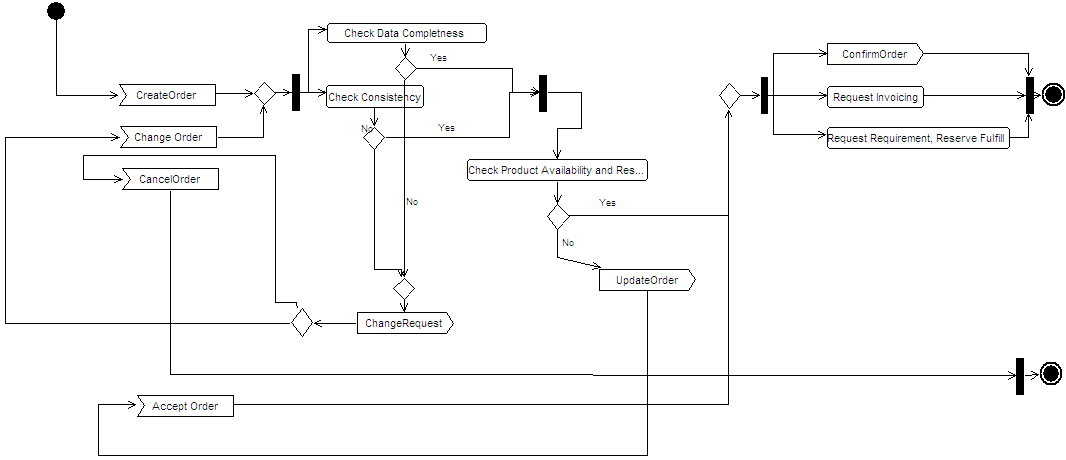
\includegraphics[width=18cm]{images/SAPExample.png}
	\caption{Exemplar Performance-Annotated UML2 Activity Diagram}
	\label{fig:SAPExample}
\end{figure}
\end{landscape}

The implementation of this case study using Epsilon consisted of two steps. In the first step, EVL was used to validate the activity diagram to ensure that the sum of probabilities of the non-deterministic transitions of each decision node is exactly 1. Listing \ref{lst:SAP.EVL} demonstrates the \emph{ProbabilitiesSumTo1} constraint specification using EVL. 

\begin{lstlisting}[basicstyle=\ttfamily\footnotesize, flexiblecolumns=true, numbers=left, nolol=true, caption=Performance-Annotated Activity Diagram Constraints using EVL, label=lst:SAP.EVL, language=EVL, tabsize=2]
import 'UML2.lib.eol';

context DecisionNode {
	
	constraint ProbabilitiesSumTo1 {
		
		guard : self.outgoing.exists(cf|cf.
			getStereotypeApplication('ExecutionProbability').
			isDefined())
		
		check {
			var sum : Real := 0;
			for (cf in self.outgoing) {
				var sa := cf.getStereotypeApplication
					('ExecutionProbability');
				if (sa.isDefined()) {
					sum := sum + sa.Probability;
				}
			}
			return sum = 1.0;
		}
		
		message : 'Sum of probabilities of decision node ' 
			+ self.name + ' is ' + sum 
		
	}
	
}
\end{lstlisting}

The next step was to simulate the execution of the model. For this purpose, non-invasive user defined operations (discussed in Section \ref{sec:Design.EOL.Operations}) were defined on the executable parts of the model using EOL. Listing \ref{lst:SAP.EOL} demonstrates the simulation specification in EOL. In line \ref{line:DecisionNode.execute} the \emph{DesicionNode.execute()} operation randomly selects one of the outgoing control flows of the decision node (based on their probabilities) and calls the \emph{walk()} operation on it. In line \ref{line:ControlFlow.walk}, the \emph{walk()} operation executes the target of the control flow. Operation \emph{Action.execute()} in line \ref{line:Action.execute} executes an action by adding its costs to the global variables defined in lines \ref{line:cpuTime} -- \ref{line:dbRows}. Finally, the \emph{JoinNode.execute()} operation defines that all incoming control flows must be first traversed before the outgoing control flows of a join-node can be executed.

\begin{lstlisting}[basicstyle=\ttfamily\footnotesize, flexiblecolumns=true, numbers=left, nolol=true, caption=Simulation using EOL, label=lst:SAP.EOL, language=EOL, tabsize=2]
import 'UML2.lib.eol';

var initialNode : InitialNode := InitialNode.allInstances().first();

var cpuTime : Integer := 0; /*@\label{line:cpuTime}@*/
var dbAccess : Integer := 0;
var dbRows : Integer := 0; /*@\label{line:dbRows}@*/
var joinNodes : new Native('java.util.HashMap');
var finished : Boolean := false;

initialNode.execute();
'Simulation trace : '.println();
('	CPUTime : ' + cpuTime).println();
('	DBAccess : ' + dbAccess).println();
('	DBRows : ' + dbRows).println();

operation DecisionNode execute() { /*@\label{line:DecisionNode.execute}@*/
	var poll : Sequence;
	for (cf in self.outgoing) {
		for (i in Sequence{0..(cf.
			getStereotypeApplication('ExecutionProbability').Probability 
			* 100).asInteger() - 1}){
			poll.add(cf);
		}
	}
	poll.random().walk();
}

operation Action execute() { /*@\label{line:Action.execute}@*/
	self.name.println();
	cpuTime := cpuTime + self.getCPUTime();
	dbAccess := dbAccess + self.getDBAccess();
	dbRows := dbRows + self.getDBRows();
	self.outgoing.first().walk();
}

operation ControlNode execute() { /*@\label{line:ControlNode.execute}@*/
	for (o in self.outgoing) {
		o.walk();
	}
}

operation JoinNode execute(cf : ControlFlow) { /*@\label{line:JoinNode.execute}@*/
	if (joinNodes.get(self).isUndefined()) {
		joinNodes.put(self, Set{cf});
	}
	else {
		joinNodes.get(self).add(cf);
	}
	if (joinNodes.get(self).size() = self.incoming.size()) {
		for (o in self.outgoing) {
			o.walk();
		}
		joinNodes.put(self, Set{});
	}
}

operation ActivityFinalNode execute() { /*@\label{line:ActivityFinalNode.execute}@*/
	finished := true;
}

operation ControlFlow walk() { /*@\label{line:ControlFlow.walk}@*/
	
	-- If a final node has been reached
	-- by some other path return
	if (finished) {return;}

	if (self.target.isTypeOf(JoinNode)){
		self.target.execute(self);
	}
	else {
		self.target.execute();
	}
}
\end{lstlisting}

A sample output of the simulation program appears in Listing \ref{lst:SAP.Output}.

\begin{lstlisting}[basicstyle=\ttfamily\footnotesize, flexiblecolumns=true, numbers=left, nolol=true, caption=Sample output of the simulation program of Listing \ref{lst:SAP.EOL}, label=lst:SAP.Output, tabsize=2]
CreateOrder
Check Data Completness
ChangeRequest
Change Order
Check Data Completness
ChangeRequest
Change Order
Check Data Completness
Check Consistency
Check Product Availability and Reserve
ConfirmOrder
Request Invoicing
Request Requirement, Reserve Fulfill
Simulation trace : 
	CPUTime : 2440
	DBAccess : 357
	DBRows : 347
\end{lstlisting}

It is worth noting that despite their different purposes, both the EVL constraints module in Listing \ref{lst:SAP.EVL} and the EOL simulation module in Listing \ref{lst:SAP.EOL} import the \emph{Uml.lib.eol} library which is displayed in Listing \ref{lst:SAP.UMLLib} to reuse the getStereotypeApplication() operation it contains.

\begin{lstlisting}[basicstyle=\ttfamily\footnotesize, flexiblecolumns=true, numbers=left, nolol=true, caption=The shared Uml.lib.eol library, label=lst:SAP.UMLLib, language=EOL, tabsize=2]
operation Element getStereotypeApplication(stereotype : String) {
	var s : Stereotype := self.getAppliedStereotypes().
		select(s|s.name = stereotype).first();
	if (s.isDefined()) {
		return self.getStereotypeApplication(s);
	}
}
\end{lstlisting}

Through this case study, the capabilities of Epsilon for programmatic model manipulation were demonstrated to the SAP team which provided positive feedback and expressed interest for further experiments in the context of performance-driven model engineering using Epsilon.

\subsection{External References}

Through a web survey, a number of external publications ( currently \cite{Zito2006,Langlois2006,Queralt2006,Boronat2006,Conmy2006,Karlsch2006,Eessaar2006,Costa2007,MinimalOCL,AlgebraicView,CrosscuttingMT,FeatureOriented,Weise2007,Pons08,Brauer2007,Rubin2008,VORA,Markovic2008,BrauerThesis,Reiter22007,Pons2007,Lazar2007,ReiterPetri2007,Zamani2007,Jeanneret2008}) in which the respective work is compared to, or uses, the work performed in the context of this thesis have been identified. This provides further evidence of the novelty of this work and its impact and acceptance in the MDE research community.

\subsection{Uses in other Projects}

\subsubsection{INESS Project}
The department of Computer Science will explore the use of Epsilon in the context of the European FP7 project ``INESS'' (Integrated European Signalling System) (starting in autumn 2008) for validation of functional requirements for rail signalling systems across Europe. This will include: capture of functional and safety requirements for rail signalling systems; simulation of these requirements; transformation of models into formal representations (e.g., in B and Circus); and generation of reports. As such, the project expects to use Epsilon languages like ETL, EGL, and EVL.

\subsubsection{SSEI Project}

In the context of the SSEI project\footnote{http://www.ssei.org.uk}, the department of Computer Science will use Epsilon for model-based systems integration, involving systems that exist solely as code (both source and binary) as well as models stored in a variety of formats. The project envisions using ECL for model comparison of both structure and behaviour; and EML for integration. Additional effort will need to be made to support the production of models from text representations; this may involve integration of components from the AMMA and openArchitectureWare platforms, or the development of new Epsilon components. 

\subsection{Internal and External Collaborations}
\label{sec:Collaborations}

The results of this work have been used in a number of internal and external collaborations. This section summarizes the most important of them.

\paragraph{University of Seville,  Group MaCMAS (Methodology for Analysing Complex MultiAgent Sytems)}

The MaCMAS group has implemented an extension to the ArgoUML modelling tool to support complex multi-agent systems. During this collaboration, their modelling tool was enhanced with support for specifying and executing Epsilon Object Language (EOL) programs which allowed the group to further automate the model refinement process.

\paragraph{Boris Gruschko, SAP, Karlsruhe}

In this work ETL was used to perform automated migration of models as a response to changes in the metamodels they conform to. The outcome of this work was presented in \cite{Gruschko2007}.

\paragraph{Philippa Conmy, HISE, York}

In this work EOL was used to perform mutation of processor-network models for failure analysis and ETL was used to transform models into a suitable format for a proprietary tool that implements FPTC (Failure Propagation Transformation Calculus).

\paragraph{George Despotou, HISE, York}

In this work, EVL constraints were used to express the constraints of a metamodel for Dependability Cases and EWL wizards were used to automate the model composition and refinement process.

\paragraph{Jules White, Vanderbilt University, Nashville}

There is ongoing work on integrating EWL with the GEMS \cite{GEMS} framework to enable execution of EWL wizards within GEMS-based editors.

\section{Evaluating Reuse}
\label{sec:Evaluation.Reuse}

The research hypothesis stated that despite their differences and task-specific requirements, \textit{...all those different model management tasks can be supported with a family of integrated task-specific languages that builds on a platform that provides a set of common reusable
features to maximize reuse, uniformity and interoperability}. To justify the claim for reuse, the amount of infrastructure functionality that can be reused when implementing task-specific languages should be considerable.

This section provides evidence about reuse metrics in the Epsilon prototype. To measure reuse, this section provides metrics of the amount of source code that has been required to provide tool-support for the base language (EOL) and the task-specific languages built atop it.

\subsection{Runtime}

Table \ref{tab:LinesOfJavaCodeLanguage} shows the total lines of code required to implement the runtime (interpreter and internal object model) of each language in the platform. These figures suggest the benefit from reuse as the size of the runtime of each task-specific language is around 50\% of the size of the shared infrastructure.

\begin{table}
	\centering
		\begin{tabular}{|l|l|}\hline
		\textbf{Language} & \textbf{Lines of Code} \\\hline
		EOL	& 13335 \\\hline
		ETL	& 6683 \\\hline
		EML	& 6878 \\\hline
		EVL	& 7216 \\\hline
		ECL	& 6804 \\\hline
		EWL	& 6169 \\\hline
		EGL	& 2609 \\\hline
		\end{tabular}		
	\caption{Lines of Java Code for each Language Runtime}
	\label{tab:LinesOfJavaCodeLanguage}
\end{table}

However, not all source code required for constructing a language runtime has been hand-crafted. Instead, a part of the code has been generated from the grammar that specifies the textual concrete syntax of each language. Table \ref{tab:LinesOfGrammarAndGeneratedCode} demonstrates the lines of code of the grammar of each language and the code generated from it by the parser generator component (which is ANTLR \cite{ANTLR} for the specific implementation).

\begin{table}
	\centering
		\begin{tabular}{|l|l|l|}\hline
		\textbf{Language} & \textbf{Grammar LOC} & \textbf{Generated LOC} \\\hline
		EOL	& 1005 &5441\\\hline
		ETL & 95 & 5962\\\hline
		EML & 64 & 6141\\\hline	
		EVL & 119 & 6400\\\hline
		ECL & 109 & 6055\\\hline	
		EWL & 74 & 5904\\\hline	
		EGL & 0 & 0\\\hline	
		\end{tabular}
	\caption{Lines of Grammar and Generated Code for each Language Runtime}
	\label{tab:LinesOfGrammarAndGeneratedCode}
\end{table}

To obtain more representative source code metrics, the size of the generated code for each language parser is replaced with the size of the grammar from which it has been automatically generated. The updated results appear in Table \ref{tab:HandCraftedCode}.

\begin{table}
	\centering
		\begin{tabular}{|l|l|}\hline
			\textbf{Language} & \textbf{Hand-Crafted Grammar and Code LOC} \\\hline
		EOL	& 8899 \\\hline
		ETL	& 816 \\\hline
		EML	& 801 \\\hline
		EVL	& 935 \\\hline
		ECL	& 858 \\\hline
		EWL	& 339 \\\hline
		EGL	& 2609 \\\hline
		\end{tabular}
	\caption{Lines of Hand-Crafted Grammar and Code for each Language Runtime}
	\label{tab:HandCraftedCode}
\end{table}

According to the results, to construct a new task-specific language, an approximate figure of 800 lines of hand-crafted Java code and ANTLR grammar is required. This figure excludes the Epsilon Generation Language (EGL) which deviates significantly by requiring almost three times as much code (2609 lines) to implement. The reason for this is that unlike the rest of the languages which are rule-based, EGL is of a radically different nature and as such it requires a considerable amount of code to accommodate the requirements of the task it has been designed for (file management, content preservation etc.).

\subsection{Development Tools (DT)}

Table \ref{tab:DTCode} provides metrics for the lines of code required for the Eclipse-based development tools (DT) of each language.

\begin{table}
	\centering
		\begin{tabular}{|l|l|l|l|}\hline
			\textbf{Language} & \textbf{Lines of DT Code} \\\hline
		EOL	& 2990\\\hline
		ETL	&	439 \\\hline
		EML	&	325 \\\hline
		EVL	&	457 \\\hline
		ECL	&	374 \\\hline
		EWL	&	552 \\\hline
		EGL	&	921 \\\hline
		\end{tabular}
	\caption{Lines of Code Required for the Development Tools}
	\label{tab:DTCode}
\end{table}

According to the figures above, the layered architecture has an impact on the amount of code required to implement development tools for task-specific languages.

Summing up the figures provided in Tables \ref{tab:HandCraftedCode} and \ref{tab:DTCode} produces the final figures of lines of code required to implement both runtime and end-user tool-support a new task-specific language are displayed in Table \ref{tab:DTAndHandCraftedCode}.

\begin{table}
	\centering
		\begin{tabular}{|l|l|l|l|}\hline
			\textbf{Language} & \textbf{Runtime LOC} & \textbf{DT LOC} & \textbf{Total LOC} \\\hline
		EOL	& 8899 & 2990 & 11889\\\hline
		ETL	&	816 & 439 & 1255\\\hline
		EML	&	801 & 325 & 1126\\\hline
		EVL	&	935 & 457 & 1392\\\hline
		ECL	&	858 & 374 & 1232\\\hline
		EWL	&	339 & 552 & 891\\\hline
		EGL	&	2609 & 921 & 3530\\\hline
		\end{tabular}
	\caption{Total Lines of Code Required for Supporting each Language}
	\label{tab:DTAndHandCraftedCode}
\end{table}

The metrics displayed in Table \ref{tab:DTAndHandCraftedCode} show that, with the exception of EGL as discussed above, implementing a new task-specific language requires 1000-1500 lines of grammar and application code which is roughly 10\% of the infrastructure code. This validates the original hypothesis that different model management tasks share a significant amount of functionality and can therefore be implemented with enhanced reuse atop a platform, such as Epsilon, that provides a common shared infrastructure.

%\subsection{Comparison with Standalone Model Management Languages}
%
%To further demonstrate the benefits of a layered approach to model management, this section provides metrics of three stand-alone model management languages that have a similar functionality and operate in the same environment (Eclipse) as Epsilon. The languages of choice were MOFScript which is a model-to-text language and ATL and TefKat which are model-to-model transformation languages. Table \ref{tab:StandaloneLanguagesMetrics} demonstrates the size of the source code of each language. More details about obtaining the metrics for these languages are provided in Appendix XXX.
%
%\begin{table}
%	\centering
%		\begin{tabular}{|l|l|l|l|}\hline
%			Language & Hand-Crafted Grammar and Code LOC & DT LOC & Total LOC \\\hline
%		MOFScript	& 9358 & 3796 & 13154\\\hline
%		ATL	&	10401 & 9027 & 19428\\\hline
%		TefKat	&	10067 & 2011 & 12078\\\hline
%		\end{tabular}
%	\caption{Total Lines of Code Required for Supporting each Language}
%	\label{tab:DTAndHandCraftedCode}
%\end{table}
%
%\begin{table}
%	\centering
%		\begin{tabular}{|l|l|l|l|}\hline
%			Language & Hand-Crafted Grammar and Code LOC & DT LOC & Total LOC \\\hline
%		ETL	&	9715 & 3429 & 13144\\\hline
%		EML	&	9700 & 3315 & 13015\\\hline
%		EVL	&	9834 & 3447 & 13281\\\hline
%		ECL	&	9757 & 3364 & 13121\\\hline
%		EWL	&	9238 & 3542 & 12780\\\hline
%		EGL	&	11508 & 3911 & 15419\\\hline
%		\end{tabular}
%	\caption{Cumulative Size of Epsilon Task-Specific Languages}
%	\label{tab:CumulativeSize}
%\end{table}

\section{Limitations and Shortcomings}
\label{sec:Evaluation.Limitations}

This section presents the main limitations and shortcomings of the proposed approach and reference implementation, explains why these limitations could not be addressed in the context of this work, and provides directions to overcoming them in future design and implementation iterations.

\subsection{Lack of Formal Execution Semantics}
\label{sec:ExecutionSemanticsEvaluation}

As discussed in Section \ref{sec:Design.EOL}, different approaches can be used to specify the execution semantics of software languages. With respect to the time constraints of this project, a decision had to be made early in the process as to whether formal semantics (e.g. translational/denotational semantics) or a reference implementation should be employed to specify the execution semantics of the languages designed within the project.

The decision to provide a reference implementation instead of a formal semantics was predominantly influenced by the setting in which the project was carried out. More specifically, the project was realized within two large EU projects (ModelWare and ModelPlex) where research results needed to be exploitable by industrial partners on their case studies. A concrete reference implementation made it possible to implement several case studies provided by industrial partners and thus, receive valuable feedback from them that has partly driven the evolution of the architecture of the platform and the individual languages to their current state. Also, through the reference implementation, Epsilon has become visible and accessible to external users through the respective Eclipse GMT component, as discussed in Section \ref{sec:GMT}. This has generated substantial feedback from external users, that has been valuable for identifying and repairing design and technical defects in the languages.

At this point it should be stressed that the aim of this discussion is to justify the choice of a reference implementation over a formal semantics under the imposed constraints, not to underrate the value of formal semantics. An established formal semantics of the languages would enable formal analysis, refinement and proof of model management programs, which are all desirable capabilities in the context of model driven engineering, particularly when used to construct safety- (and otherwise) critical systems.

\section{Reference Implementation}
\label{sec:Evaluation.ReferenceImplementation}

This aim of this section is to evaluate the reference implementation that has been realized to examine the validity of the hypothesis. 

As examples of hierarchically layered families of languages, particularly on model management, are practically non-existent in the literature, it was realized early in the process that defining the final syntax and semantics of the languages would require many change cycles - as it eventually has.

To reduce ripple effects triggered by frequent changes in the languages, the architecture and technical design of the platform were predominantly driven by modifiability and extensibility. Therefore, the reference implementation intentionally fails to provide support for lower priority - but nevertheless useful - features such as static type checking, context-sensitive editing features and debugging support.

Extensive ripple effects introduced by such facilities would influence the evolution of the languages negatively since they would require significant effort to address and thus gradually become a burden for experimenting with novel features that would require changes to the syntax and the semantics of the languages. This intuition proved to be reasonable during the development life-cycle of the languages and their supporting tools. Due to its flexibility, the established architecture enabled experimentation with novel features such as user-interactivity, transactions and native-object access without significant ripple effects. 

Nevertheless, the flexible architecture of the implementation has had an impact on performance and usability. By choosing a lightweight interpreter-based approach instead of a compiler-based approach, the runtime performance of the languages is impacted negatively, as expected. Moreover, the development tools lack productivity features such as automated support for refactoring and coding assistance which are important for large-scale industrial use.

Overall, the trade-off between flexibility and performance/usability is considered to be fair as the purpose of the project was not to produce industrial strength tools, but to validate the hypothesis that a layered platform of languages with emphasis on reuse, uniformity and consistency can be used to address diverse model management tasks in a meaningful way.

\section{Chapter Summary}

This chapter has confirmed the validity of the hypothesis stated in Chapter \ref{chp:Analysis} using a number of criteria such as: applicability in a complex externally-defined case study, reuse metrics, publications and acceptance by the research community, establishment of a user community, internal and external collaborations, and use of the reference implementation for several case studies in the context of the ModelWare and ModelPlex research projects.

The evaluation has demonstrated significant benefits in terms of applicability, reuse, modularity and interoperability and has identified limitations such as the lack of a formal semantics and the need for more sophisticated development tools.